\documentclass[11pt]{article}

% --- packages (all standard; compiles on stock TeX Live / Overleaf) ---------
\usepackage[margin=1in]{geometry}
\usepackage[T1]{fontenc}
\usepackage{lmodern}
\usepackage{amsmath,amssymb,amsthm}
\usepackage{booktabs}
\usepackage{graphicx}
\usepackage{xcolor}
\usepackage{caption}
\usepackage[hidelinks]{hyperref}
\usepackage{microtype}

\graphicspath{{figures/}}

\theoremstyle{plain}
\newtheorem{conjecture}{Conjecture}
\theoremstyle{definition}
\newtheorem{definition}{Definition}
\theoremstyle{remark}
\newtheorem{remark}{Remark}

\newcommand{\Pself}{P_{\mathrm{self}}}
\newcommand{\Pneu}{P_{\mathrm{neu}}}
\newcommand{\tbd}{\textcolor{red}{\textbf{[TBD]}}}

\title{\bfseries Context Contagion in Real Transformers:\\[2pt]
A Progress Report}
\author{Dan Shumow\thanks{Work-in-progress write-up of the open-source project
\texttt{transformer-context-contagion}, the empirical follow-on to the toy-model analyses
\texttt{trust-is-the-attack-surface}. All numbers and figures are reproduced by the
\texttt{experiments/} scripts in that repository; the running log is \texttt{results\_log.md}.}}
\date{June 2026 --- \emph{draft, in progress}}

\begin{document}
\maketitle

\begin{abstract}
Two companion analyses~\cite{shumow2026trust,shumow2026contagion} establish, \emph{exactly}
on a toy global-plus-cache Markov model, that in-context exploitability tracks \emph{trust}
rather than usefulness, and that self-reproducing token strings (\emph{quines}) can be
planted in a cache, hijack an occupied one, and spread between caches as a
context-window worm---all cheapest and most transmissible under a longest-match
(\emph{induction-head}) surrogate. Those results were stated as \emph{conjectures} for real
transformers. This report is the running status of testing them on real models. So far we
have built the harness and run the first two stages of the keystone experiment on
GPT-2-small. We find (i) a clear \emph{condensation knee}: a repeated out-of-distribution
string begins to be regenerated past a sharp threshold in the repetition count, with the
threshold \emph{decreasing} in string length (the induction-like, length-robust signature,
opposite of fixed-order brittleness); and (ii) that reproduction is predominantly
\emph{cue-dependent}---a non-matching prime mostly fails to elicit the string while a
matching one reliably does---a behavioral induction signature obtained without
interpretability tooling; and (iii) confirmed \emph{mechanistically} that the model's own
induction heads carry it---ablating the canonical GPT-2 induction heads collapses
reproduction near the knee, far beyond random-head damage. Controls further show the knee
is a repetition (not context-length) effect though distance-sensitive, and the phenomena
replicate in a second model family (Pythia). We then confirm the three downstream claims:
\emph{(iv)} poisonability tracks \emph{trust}, not usefulness---repetitive gibberish is fully
poisonable while useful non-repetitive prose is not ($\mathrm{corr}(P,\text{useful}){=}{-}0.20$
vs.\ $\mathrm{corr}(P,\text{trust}){=}{+}0.54$, C4); \emph{(v)} a payload planted in a document
hijacks generation only when recent \emph{and} sufficiently repeated---delivery factors as
entry$\,\times\,$lock-in (C5); and \emph{(vi)} output fed back as another context propagates
as a \emph{worm} with a critical string length (short strings reach an endemic load, long ones
die out) and a \emph{cross-tokenizer firebreak} (GPT-2$\to$Pythia transmission collapses, C6).
A \emph{paired detector} closes the loop: scoring contexts by induction-trust on repeated spans
separates poisoned from clean documents perfectly (AUC $1.0$) and flags the poisonable
configuration before it crosses the hijack knee---the transformer realization of the toy's
\emph{bound-trust} defense. We then take the keystone to \emph{scale} on a cloud GPU: the
condensation knee is low and length-robust across \mbox{355M--7B} in four model families and
essentially \emph{flat with parameter count}---the copy mechanism is saturated by 355M (C3)---and
it \emph{persists in instruction-tuned/chat models}, which copy rather than refuse, with only a
modest threshold increase (E1.3/E1.4, \S\ref{sec:scale}). What remains is the mechanistic
attribution \emph{at scale} (induction-head ablation on $\ge$24\,GB models) and the
larger-context, retrieval-grounded versions of the downstream claims.
\end{abstract}

% ===========================================================================
\section{Scope and status}\label{sec:status}
% ===========================================================================
This is a \emph{progress report}, not a finished paper: sections marked \tbd\ are planned
but not yet run. The conceptual framing, the exact toy results, and the falsifiable
conjecture all live in the companion write-ups~\cite{shumow2026trust,shumow2026contagion};
we recap only what is needed. The threat is concrete---context poisoning and
self-replicating prompts already target real retrieval-augmented and agent
pipelines~\cite{greshake2023,cohen2024}---and the toy substrate is a from-scratch analogue
of the parametric-versus-in-context split studied by Bietti et al.~\cite{bietti2023}. The
detailed experiment plan (claims, controls, statistics,
phasing) is the repository's \texttt{transformer\_validation\_plan.md} and
\texttt{e1\_plan.md}; this report records what those plans have produced so far.

\begin{table}[h]
\centering\small
\begin{tabular}{llp{0.46\textwidth}}
\toprule
Stage & Status & What \\
\midrule
E1.0 smoke test & done & knee exists on GPT-2 (qualitative). \\
E1.1 measured knee & done & knee vs length with controls + CIs (\S\ref{sec:e1}). \\
E1.2 copy vs.\ frequency & done & cue-dependence; behavioral induction (\S\ref{sec:e1b}). \\
E1.5 context confound & done & knee is an $N$ effect; distance-sensitive (\S\ref{sec:e15}). \\
E1.3 size sweep & partial & cross-family replication; 8\,GB caps it at $\le$162M (\S\ref{sec:e13}). \\
E2 induction attribution & done & induction heads \emph{causally} carry it (\S\ref{sec:e2}). \\
E4-lite trust, not usefulness & done & poisonability $\perp$ usefulness, $\parallel$ trust (\S\ref{sec:e4}). \\
E5-lite delivery in a document & done & hijack $=$ entry $\times$ lock-in (\S\ref{sec:e5}). \\
E6 the worm / $R_0$ & done & critical length; cross-tokenizer firebreak (\S\ref{sec:e6}). \\
E7 paired detector & done & flags poisonable repeated spans, AUC $1.0$ (\S\ref{sec:e7}). \\
E1.4 modern / chat models & done & knee persists in chat models, base$\to$instruct (\S\ref{sec:scale}). \\
E1.3 size sweep ($\ge$355M) & done & knee flat with scale, 355M--7B, 4 families (\S\ref{sec:scale}). \\
E2 attribution at scale & \tbd & induction-head ablation on $\ge$24\,GB models. \\
\bottomrule
\end{tabular}
\caption{Status of the experimental program. Stage numbering follows
\texttt{transformer\_validation\_plan.md} and \texttt{e1\_plan.md}.}
\label{tab:status}
\end{table}

% ===========================================================================
\section{Claims under test}\label{sec:claims}
% ===========================================================================
Each maps a toy object to a transformer-measurable quantity; see the plan for the full
list and the experiments E1--E6.

\begin{table}[h]
\centering\small
\begin{tabular}{clp{0.44\textwidth}}
\toprule
& Toy result & Real-transformer prediction \\
\midrule
C1 & condensation knee & a repeated OOD string is regenerated past a sharp threshold in $N$ \\
C2 & induction is the engine & reproduction is carried by induction heads (copy-on-match) \\
C3 & length penalty vanishes under induction & knee location roughly flat or \emph{decreasing} in length \\
C4 & exploitability tracks trust, not usefulness & repetitive contexts most poisonable, $\approx$ independent of benefit \\
C5 & delivery $=$ entry $\times$ lock-in & a planted span hijacks generation in a long context \\
C6 & worm with $R_0\approx T/(p\,k_{\mathrm{thresh}})$ & output fed back propagates; short strings spread, long die \\
\bottomrule
\end{tabular}
\caption{The conjecture, claim by claim. All six now have a real-transformer result on
GPT-2-small: \textbf{C1}, \textbf{C3} (\S\ref{sec:e1}); \textbf{C2} behaviorally (\S\ref{sec:e1b})
and mechanistically (\S\ref{sec:e2}); \textbf{C4} (\S\ref{sec:e4}); \textbf{C5} (\S\ref{sec:e5});
\textbf{C6} (\S\ref{sec:e6}). What remains is scale (size sweep, instruct models).}
\label{tab:claims}
\end{table}

% ===========================================================================
\section{Method}\label{sec:method}
% ===========================================================================
\paragraph{Payloads.} A \emph{payload} is a short cyclic string $S$ of token ids the model
would essentially never emit on its own, so any reproduction is the copy mechanism, not the
model's taste---the analogue of the toy's rainbow / de Bruijn quines. Payloads are built at
the \emph{token} level (length $p$ is in tokens) from a pool of rare, round-trip-stable
single tokens, as distinct-token (``rainbow'') cycles. We use $R$ independent random
payloads per length and average, with Wilson confidence intervals.

\paragraph{Scoring.} Reproduction is scored at the level of \emph{transitions}, not
positions: a single slip only phase-shifts a positional comparison and tanks all later
positions even while the model is faithfully reproducing. Given $S$ and a generated
continuation, the per-step fidelity is the fraction of steps obeying $S$'s successor rule
given the realized window; a continuation \emph{reproduces} $S$ if that fidelity exceeds
$\tfrac12$. $P(\text{reproduce})$ is the fraction of sampled continuations that do.

\paragraph{Controls.} Three controls separate genuine pattern-copying from artifacts:
(i) a \emph{no-payload} ($N{=}0$) control---prime at the same start token but never show
the payload---measures spontaneous emission, which must be $\approx 0$; (ii) a
\emph{scrambled} control---the same tokens in shuffled order, destroying the repeated
$n$-gram while preserving token frequencies; (iii) a \emph{cue} control (\S\ref{sec:e1b})
contrasting a matching with a non-matching generation prompt.

\paragraph{Setup.} Results below are GPT-2-small (124M)~\cite{radford2019}, on an Apple-Silicon
laptop (MPS/Metal backend), \texttt{torch~2.8}, \texttt{transformers~4.57}, sampled at
temperature $1.0$. This is a development-scale environment: it establishes the phenomena on
one small model; the size sweep (E1.3) needs more compute.

% ===========================================================================
\section{E1.1: the condensation knee}\label{sec:e1}
% ===========================================================================
We sweep the repetition count $N$ and the string length $p$, estimating
$P(\text{reproduce})$ over $R{=}4$ payloads $\times 10$ sampled continuations per cell, with
the scrambled and no-payload controls and a bootstrap interval on the knee location $N^*$
(the interpolated $P{=}\tfrac12$ crossing).

\begin{figure}[t]
\centering
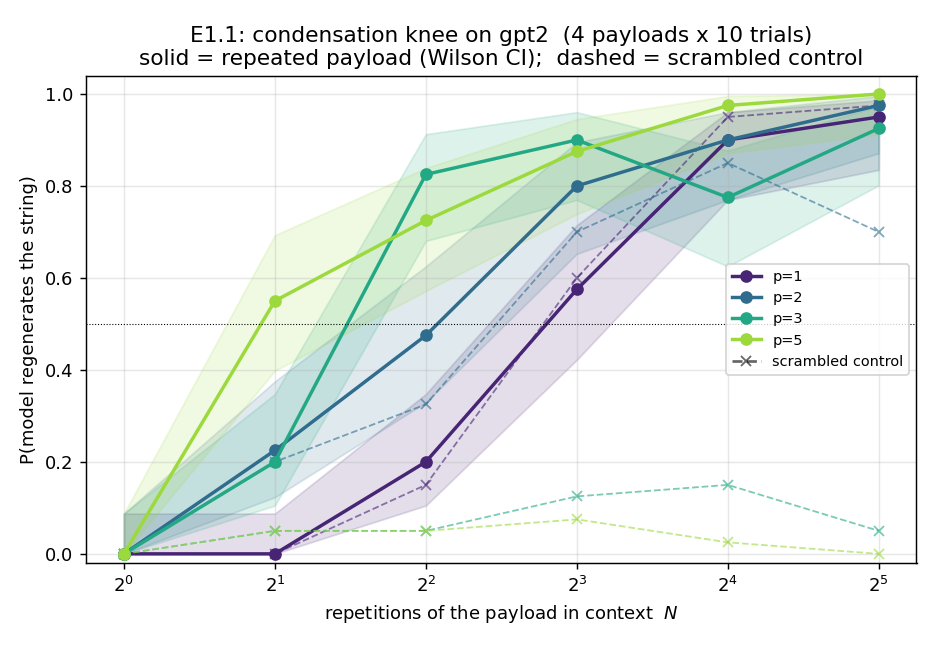
\includegraphics[width=0.74\textwidth]{e1_1_knee_gpt2.png}
\caption{$P(\text{reproduce})$ vs.\ repetition count $N$ on GPT-2-small, per string length
(solid, with Wilson bands); dashed is the scrambled control. A clear knee in $N$ exists for
every length. Reproduced by \texttt{experiments/e1\_condensation\_knee.py}.}
\label{fig:knee}
\end{figure}

\begin{table}[h]
\centering\small
\begin{tabular}{ccccc}
\toprule
$p$ & knee $N^*$ (95\% CI) & width & scrambled $P$ @ $N{=}32$ & no-payload $P$ \\
\midrule
1 & 7.2 (5.5--10.3) & 7.8 & \textbf{0.97} & 0.00 \\
2 & 4.3 (1.7--6.2)  & 5.2 & \textbf{0.70} & 0.00 \\
3 & 3.0 (2.6--3.6)  & 1.6 & 0.05 & 0.00 \\
5 & 1.9 (1.7--4.8)  & 3.2 & 0.00 & 0.00 \\
\bottomrule
\end{tabular}
\caption{E1.1 on GPT-2-small. The knee $N^*$ decreases with length; the no-payload control
is $0$ throughout; the scrambled control is near $0$ for $p\ge3$ but \emph{not} for short
$p$ (see text).}
\label{tab:e1}
\end{table}

\paragraph{C1 (the knee exists): confirmed.} Every length shows a clear threshold in $N$
(Figure~\ref{fig:knee}), and the no-payload control is $0.00$ everywhere
(Table~\ref{tab:e1})---the payloads are genuinely out-of-distribution, so reproduction is
caused by the repetitions, not the model's prior.

\paragraph{C3 (length robustness): confirmed, and stronger than ``flat.''} $N^*$
\emph{decreases} with length, $7.2\to4.3\to3.0\to1.9$ (Figure~\ref{fig:nstar}): longer
strings are \emph{easier} to plant. This is the induction-like signature---the opposite of
the fixed-order count cache's doubly-exponential brittleness ladder~\cite{shumow2026contagion}.

\paragraph{The scrambled control exposed a length-dependent mechanism.} For $p\ge3$ the
scrambled control stays near $0$ while the payload locks: reproduction needs the
\emph{pattern}. But for $p\le2$ the scrambled control reproduces almost as well
($0.97,0.70$), because it is \emph{degenerate} at short length---a single repeated token has
no order to scramble, and a bigram re-forms by chance. This motivated E1.2, which separates
copying from frequency directly.

\begin{figure}[t]
\centering
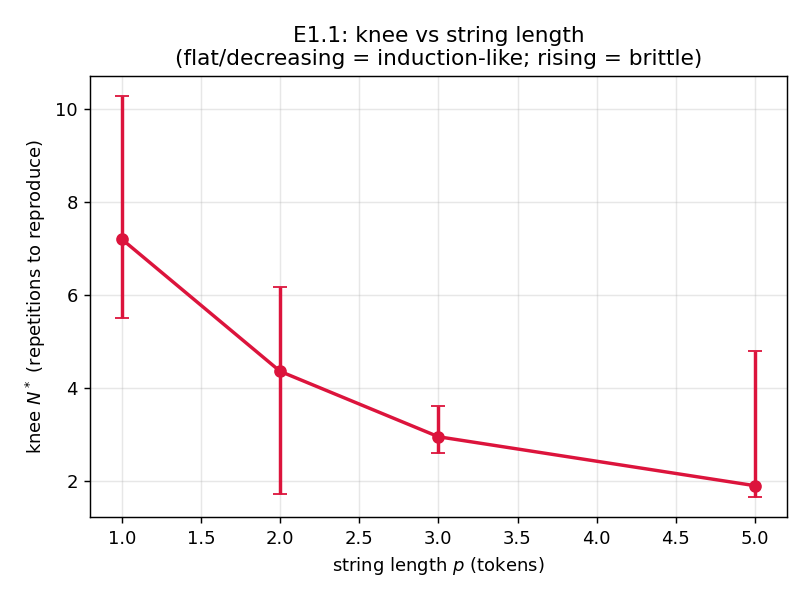
\includegraphics[width=0.56\textwidth]{e1_1_Nstar_gpt2.png}
\caption{Knee $N^*$ vs.\ string length (bootstrap CI). Decreasing $N^*$ is the
induction-like, length-robust behavior; a rising curve would indicate fixed-order
brittleness.}
\label{fig:nstar}
\end{figure}

% ===========================================================================
\section{E1.2: copy versus frequency}\label{sec:e1b}
% ===========================================================================
Is reproduction genuine copy-on-match (induction) or a frequency bias (the repeated tokens
simply become likely)? We separate them behaviorally---no activation access. After
streaming $S$ a fixed above-knee number of times $N$, we prime generation two ways:
a \emph{self-cue} at $S$'s own tail (a matching cue), and a \emph{neutral-cue} appending a
fresh token $z\notin S$ (a non-matching cue), and compare $P(\text{reproduce }S)$. Induction
is cue-triggered (the matching cue reproduces, the non-matching one should not); a frequency
bias is cue-independent. The signature is the gap $\Pself-\Pneu$ vs.\ length.

\begin{table}[h]
\centering\small
\begin{tabular}{ccccc}
\toprule
$p$ & $\Pself$ & $\Pneu$ & gap ($N{=}16$) & gap ($N{=}32$) \\
\midrule
1 & 0.78--0.92 & \textbf{0.26--0.29} & $+0.51$ & $+0.62$ \\
2 & 0.92--0.97 & 0.07--0.12 & $+0.79$ & $+0.90$ \\
3 & 0.97--1.00 & 0.07--0.19 & $+0.90$ & $+0.81$ \\
5 & 1.00       & 0.17--0.32 & $+0.83$ & $+0.68$ \\
8 & 0.99--1.00 & 0.15--0.26 & $+0.85$ & $+0.72$ \\
\bottomrule
\end{tabular}
\caption{E1.2 on GPT-2-small ($R{=}6$ payloads $\times 12$ trials). The matching cue locks;
the non-matching cue mostly fails. The gap is large at every length and smallest at $p{=}1$.}
\label{tab:e1b}
\end{table}

\begin{figure}[t]
\centering
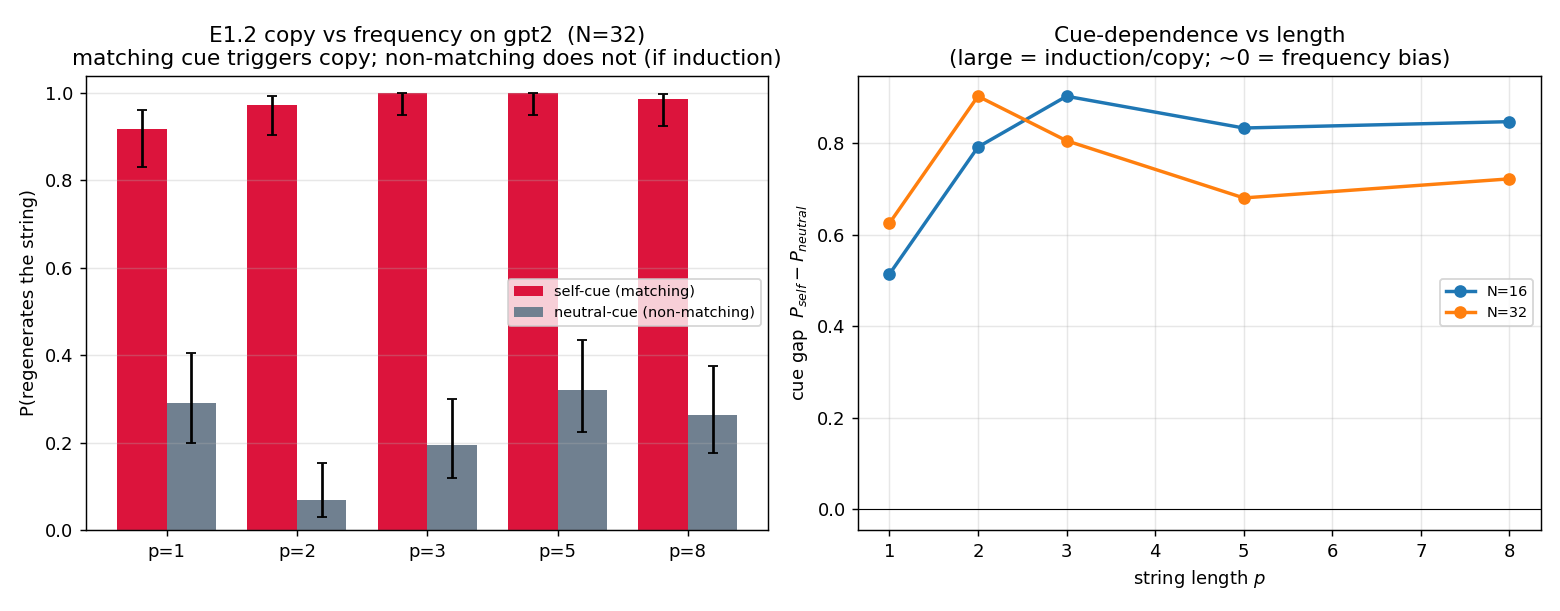
\includegraphics[width=\textwidth]{e1_2_gpt2.png}
\caption{Copy vs.\ frequency. \emph{Left:} matching (self) vs.\ non-matching (neutral) cue
at $N{=}32$ per length, Wilson CIs. \emph{Right:} the cue gap $\Pself-\Pneu$ vs.\ length;
large everywhere (cue-triggered copy), smallest at $p{=}1$ (largest frequency tail).
Reproduced by \texttt{experiments/e1\_2\_cue.py}.}
\label{fig:cue}
\end{figure}

\paragraph{Reproduction is predominantly cue-dependent at every length}
(Table~\ref{tab:e1b}, Figure~\ref{fig:cue}): the non-matching cue mostly fails
($\Pneu\le\!\sim\!0.3$) while the matching cue locks ($\Pself\approx0.8$--$1.0$), a gap of
$0.5$--$0.9$ well above zero. This is a behavioral induction~\cite{olsson2022}
(copy-on-match) signature, established without interpretability tooling and consistent with C2.

\paragraph{This revises the E1.1 reading.} Even $p{=}1$ is mostly copy (gap $+0.5$--$0.6$),
not the pure-frequency regime E1.1's degenerate control suggested; it merely carries the
\emph{largest frequency tail} ($\Pneu\approx0.27$, versus $\sim0.1$--$0.2$ for longer
strings), since a single token has the biggest cue-independent pull and more distinct tokens
dilute any one token's frequency. The length axis is therefore
\emph{copy-dominant-everywhere with a frequency tail largest at $p{=}1$}, not a clean regime
switch.

\begin{remark}[$\Pneu$ over-states frequency]
After the non-matching cue the model can still re-enter $S$ if it emits an $S$-token by
chance and induction then completes the pattern (the toy's re-entry / self-healing). So
$\Pneu$ is an \emph{upper} bound on the pure-frequency component, and the true copy fraction
is if anything larger than the gap suggests.
\end{remark}

% ===========================================================================
\section{E1.5: is the knee an $N$ effect or a context-length effect?}\label{sec:e15}
% ===========================================================================
E1.1's context is $S\times N$, so the number of repetitions and the total context length
grow together. E1.5 disentangles them. \emph{Test 1} compares a \emph{growing} context
($S\times N$) against a \emph{fixed} total length (filler padded to a constant length) at
each $N$. The two curves largely coincide (Figure~\ref{fig:context}, left): at fixed total
length the threshold still rises sharply with $N$, so \textbf{the knee is predominantly an
$N$ effect}, not an artifact of longer context. A secondary \emph{dilution} effect remains
(padding at low $N$ modestly lowers reproduction, strongest for longer $p$). \emph{Test 2}
holds $N$ above the knee and inserts a gap of $G$ neutral tokens between the payload and a
re-presented matching cue. Reproduction \textbf{decays with distance}---gone by
$G\approx16$--$32$ tokens for $p\ge3$ (Figure~\ref{fig:context}, right). So in GPT-2-small
the copy is recency-modulated, not arbitrarily long-range; a payload buried deep in a long
context is much weaker than one near the end. (The gap is filled with rare tokens, so part
of the decay may be filler competition rather than pure distance; larger models with
longer-range induction should push the limit out.)

\begin{figure}[t]
\centering
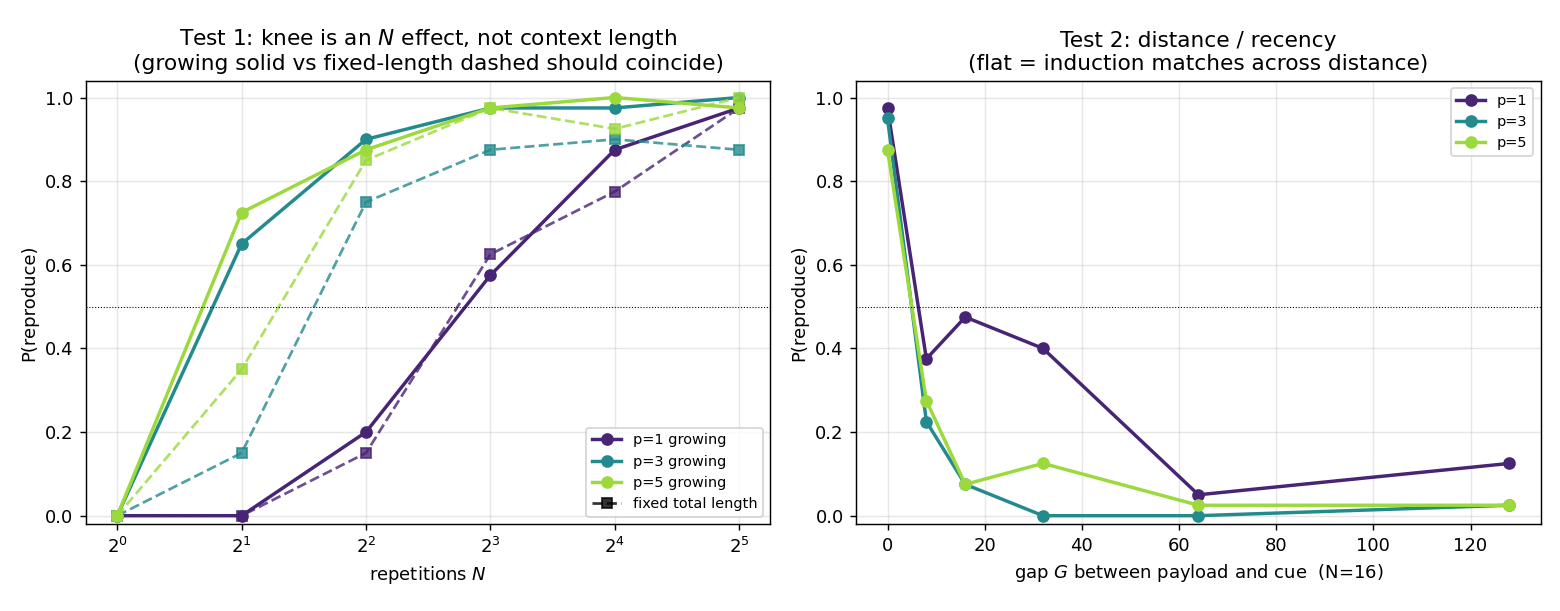
\includegraphics[width=\textwidth]{e1_5_gpt2.png}
\caption{E1.5. \emph{Left:} growing (solid) vs.\ fixed total length (dashed) -- the knee
persists at fixed length, so it is an $N$ effect. \emph{Right:} reproduction decays as the
payload is separated from the cue by a gap of $G$ neutral tokens (recency-modulated).
Reproduced by \texttt{experiments/e1\_5\_context.py}.}
\label{fig:context}
\end{figure}

% ===========================================================================
\section{E1.3-lite: cross-family replication, and an 8\,GB wall}\label{sec:e13}
% ===========================================================================
A size sweep over GPT-2 \{small, medium, large\} and Pythia \{160M, 410M\} was intended.
The dominant outcome was a \emph{hardware} one: on an 8\,GB machine, gpt2-medium (355M) and
larger thrash on swap (gpt2-large, 3\,GB of weights, ran 47 wall-minutes using $\sim$9 CPU
minutes and completed nothing). Only GPT-2-small (124M) and Pythia-160M (162M) run cleanly,
so a genuine size-scaling sweep is \textbf{deferred to more compute}. What did run shows the
condensation knee and its length-robustness ($N^*$ decreasing with $p$) in \emph{both} model
families (Figure~\ref{fig:size}), a modest cross-family generality check; the GPT-2 knees
also replicate E1.1. Pythia-160M does not lock a single token within $N\le32$ (no knee at
$p{=}1$), i.e.\ it is harder to frequency-drive than GPT-2, consistent with E1.2. The
``knee vs.\ parameters'' panel spans only two near-identical sizes and is \emph{not} a
scaling result.

\begin{figure}[t]
\centering
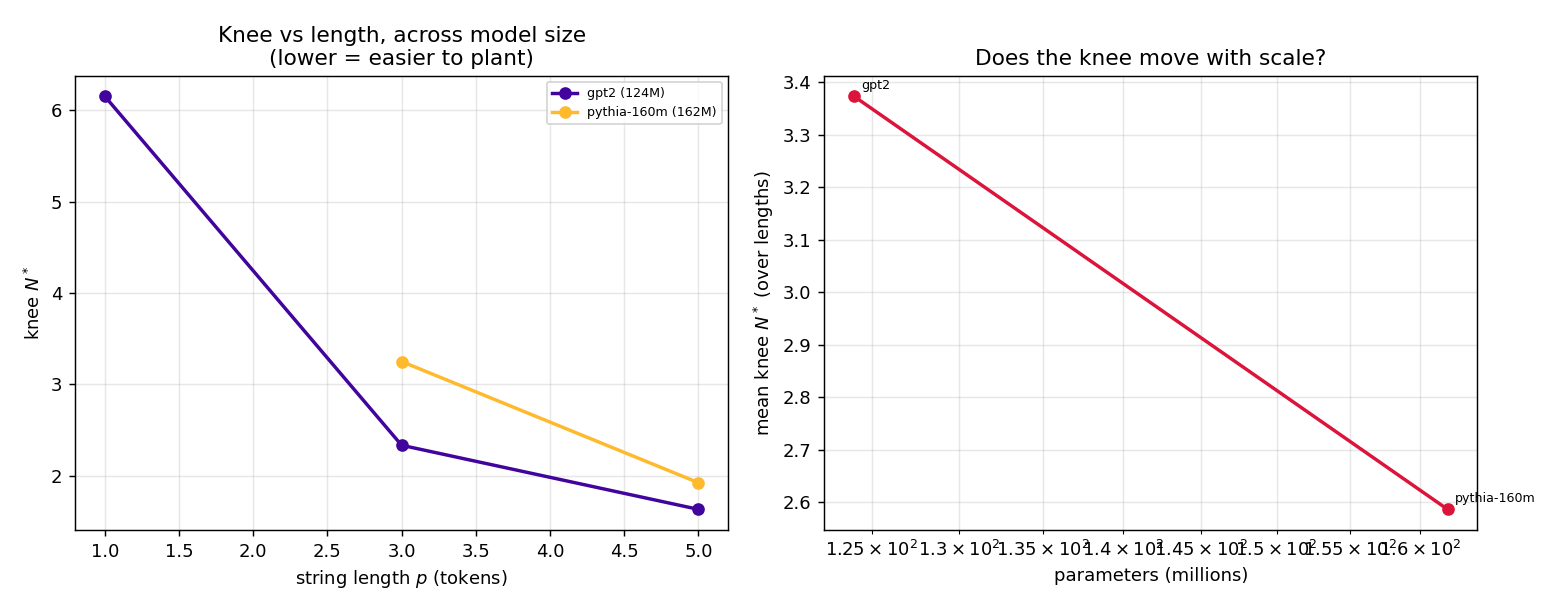
\includegraphics[width=0.86\textwidth]{e1_3.png}
\caption{E1.3-lite. \emph{Left:} the knee decreases with length in both GPT-2 and Pythia
(cross-family replication). \emph{Right:} two near-identical sizes -- not a scaling result;
a real sweep needs $>$8\,GB. Reproduced by \texttt{experiments/e1\_3\_size\_sweep.py}.}
\label{fig:size}
\end{figure}

% ===========================================================================
\section{At scale: the knee from 355M to 7B, base and chat (E1.3/E1.4)}\label{sec:scale}
% ===========================================================================
The size sweep the 8\,GB machine blocked (\S\ref{sec:e13}) was re-run on an Azure
NC4as\_T4\_v3 (NVIDIA T4, 16\,GB), in \texttt{float16}, across \textbf{twelve base models in
four families spanning 355M--7B}---GPT-2 \{medium, large, xl\}, Pythia \{410M, 1.4B, 2.8B\},
Qwen2.5 \{0.5B, 1.5B, 3B, 7B\}, Llama-3.2 \{1B, 3B\}---and then on four
\textbf{instruction-tuned} models (E1.4). Main condition only (controls validated on
GPT-2-small); knee $N^*(p)$ for $p\in\{1,3,5,8\}$, $N\in\{1,\dots,32\}$.

\begin{figure}[t]
\centering
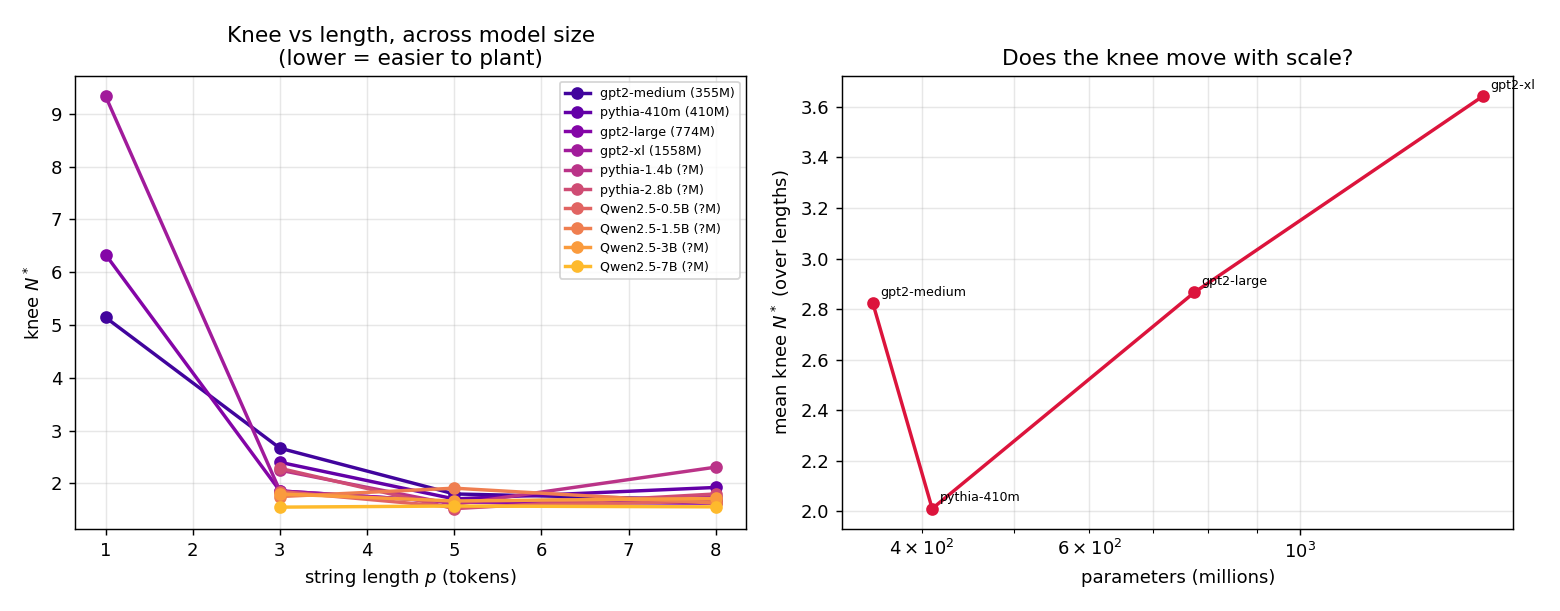
\includegraphics[width=0.86\textwidth]{e1_3_scale.png}
\caption{E1.3 at scale. \emph{Left:} knee $N^*$ vs.\ string length for each model---low and
roughly flat for $p\ge3$ at every size and in all four families. \emph{Right:} mean knee vs.\
parameters---no downward trend for $p\ge3$; the copy mechanism is already saturated by 355M.
Reproduced by \texttt{experiments/e1\_3\_size\_sweep.py}.}
\label{fig:scale}
\end{figure}

\begin{table}[h]
\centering\small
\begin{tabular}{lccccc}
\toprule
model & params & $N^*(p{=}1)$ & $p{=}3$ & $p{=}5$ & $p{=}8$ \\
\midrule
GPT-2-medium & 355M & 5.1 & 2.7 & 1.8 & 1.7 \\
GPT-2-large  & 774M & 6.3 & 1.9 & 1.6 & 1.6 \\
GPT-2-xl     & 1.5B & 9.3 & 1.9 & 1.6 & 1.7 \\
Pythia-410m  & 410M & --  & 2.4 & 1.7 & 1.9 \\
Pythia-1.4b  & 1.4B & --  & 2.3 & 1.6 & 2.3 \\
Pythia-2.8b  & 2.8B & --  & 2.3 & 1.5 & 1.8 \\
Qwen2.5-0.5B & 0.5B & --  & 1.8 & 1.5 & 1.7 \\
Qwen2.5-1.5B & 1.5B & --  & 1.8 & 1.9 & 1.6 \\
Qwen2.5-3B   & 3B   & --  & 1.8 & 1.7 & 1.7 \\
Qwen2.5-7B   & 7B   & --  & 1.5 & 1.6 & 1.6 \\
Llama-3.2-1B & 1B   & --  & 1.9 & 2.7 & 1.9 \\
Llama-3.2-3B & 3B   & --  & 1.7 & 1.9 & 1.6 \\
\bottomrule
\end{tabular}
\caption{E1.3 size sweep (Track B, T4). ``--'' $=$ no knee ($P<\tfrac12$ for $N\le32$). The
$p\ge3$ knee is low ($N^*\!\approx\!1.5$--$2.7$) and essentially size-independent.}
\label{tab:scale}
\end{table}

\paragraph{C3 holds across scale and family.} For $p\ge3$ the knee is low and roughly flat
everywhere ($N^*\!\approx\!1.5$--$2.7$, decreasing in $p$): a novel span of $\ge3$ tokens
locks in after $\sim$2 presentations at every size up to 7B and in all four families
(Fig.~\ref{fig:scale}). Induction-style length-robustness is not a small-model artifact.

\paragraph{The knee does not fall with scale.} Contrary to the loose expectation that larger
models give a lower or sharper knee, $N^*(p\ge3)$ is essentially flat in parameter count---the
copy mechanism is already saturated by 355M. Any size dependence lives in \emph{single-token}
lock-in: only the GPT-2 family locks $p{=}1$ within $N\le32$, and its knee \emph{rises} with
size ($5.1\to6.3\to9.3$). This sharpens E1.2's reading---$p{=}1$ reproduction is a
model-specific frequency-prior effect, not induction, while the induction-carried $p\ge3$ knee
is universal.

\paragraph{E1.4: instruction-tuning does not immunize.} The worry that chat models would
refuse or summarize rather than copy did not materialize: all four ran clean and reproduced
the planted span, with the knee in the same low regime (Table~\ref{tab:instruct}).
Instruction-tuning \emph{raises} the threshold modestly---most for Llama-3.2-3B-Instruct
($p{=}5$ knee $6.3$ vs.\ base $1.9$, the most resistant chat model)---but never removes it.
The small instruct model gemma-2-2b-it is the most eager copier and the only model in either
sweep to lock a \emph{single} token ($p{=}1$, $N^*{=}1.0$). C1/C3 thus extend to the realistic
chat condition.

\begin{table}[h]
\centering\small
\begin{tabular}{lcccccc}
\toprule
instruct model & params & $N^*(p{=}1)$ & $p{=}3$ & $p{=}5$ & $p{=}8$ & base $N^*(3/5/8)$ \\
\midrule
Qwen2.5-1.5B-Instruct & 1.5B & --  & 2.8 & 2.8 & 2.0 & 1.8 / 1.9 / 1.6 \\
Qwen2.5-7B-Instruct   & 7B   & --  & 1.6 & 2.5 & 1.8 & 1.5 / 1.6 / 1.6 \\
Llama-3.2-3B-Instruct & 3B   & --  & 3.2 & 6.3 & 2.0 & 1.7 / 1.9 / 1.6 \\
gemma-2-2b-it         & 2B   & 1.0 & 3.0 & 1.8 & 1.4 & --- \\
\bottomrule
\end{tabular}
\caption{E1.4 instruct models (Track B, T4), with base counterparts from
Table~\ref{tab:scale}. The knee persists; instruction-tuning raises it modestly, most for
Llama-3.2-3B-Instruct. Raw-context format (span as bare tokens, not a chat template).}
\label{tab:instruct}
\end{table}

\paragraph{Setup.} \texttt{float16} keeps the 7B models at $\sim$14\,GB on the 16\,GB T4;
gated weights (Llama, Gemma) load from cache offline. The mechanistic attribution at scale
(E2 on a $\ge$24\,GB GPU) and the coherent self-extraction capstone (E8) remain---the
24\,GB-GPU stage.

% ===========================================================================
\section{E2: induction-head attribution}\label{sec:e2}
% ===========================================================================
E1.2 showed reproduction is cue-triggered copy (behavioral induction); E2 asks whether the
model's actual induction heads carry it. Run on CPU (TransformerLens warns MPS may be
silently incorrect on torch~2.8). First, the standard repeated-random-sequence induction
score flags the top heads as \textbf{L5H5, L7H10, L6H9, L5H1, L7H2} (then L9H6, L10H1,
L9H9)---exactly the canonical GPT-2-small induction heads, validating the detector. Then a
causal test: build $S\times N$, measure $P(\text{correct next payload token})$, and ablate
the 8 induction heads versus 8 random heads, sweeping $N$.

The clean signal lives \emph{near the knee}, not at saturation: at $N{=}16$ the copy is
over-determined (many repetitions, redundant heads) and robust to losing 8 heads, but near
threshold the circuit is load-bearing. Ablating the induction heads then \textbf{collapses}
reproduction---e.g.\ at $N{=}2$, $p{=}3$: $0.40\to0.05$ ($-87\%$); $p{=}5$: $0.48\to0.09$
($-81\%$)---far beyond the $\sim$15--25\% general degradation from ablating random heads
(Figure~\ref{fig:e2}). This is the \textbf{mechanistic confirmation of C2}: the
real-transformer condensation knee is an induction-head phenomenon. (Caveats: random-head
ablation is not exactly zero, so the load-bearing signal is the induction-vs-random
\emph{differential}; 8 heads is a subset of the circuit; GPT-2-small only.)

\begin{figure}[t]
\centering
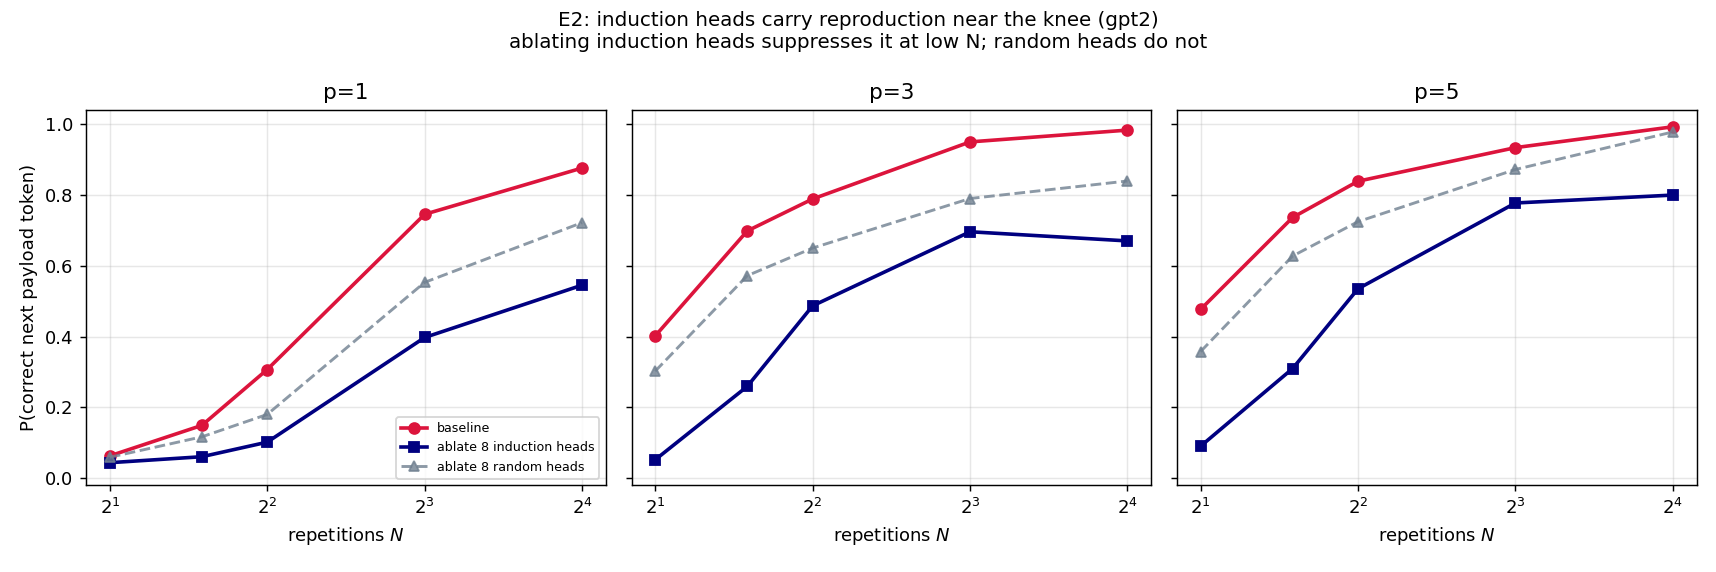
\includegraphics[width=\textwidth]{e2_gpt2.png}
\caption{E2. Per length, $P(\text{correct next token})$ vs.\ $N$ for baseline, ablating 8
induction heads, and ablating 8 random heads. Induction ablation suppresses reproduction
far below baseline and below random ablation, most strongly near the knee (low $N$).
Reproduced by \texttt{experiments/e2\_induction.py}.}
\label{fig:e2}
\end{figure}

% ===========================================================================
\section{E4-lite: poisonability tracks trust, not usefulness}\label{sec:e4}
% ===========================================================================
The toy's headline (C4) is that exploitability follows how much the model \emph{trusts} a
span, not how \emph{useful} it is. We test the dissociation with a $2\times2$ of contexts---
\{repetitive, non-repetitive\} $\times$ \{useful (real text), useless (OOD gibberish)\}---each
scored on three axes: usefulness $U$ (naturalness $=$ mean log-prob of one content unit),
trust $T$ (induction-head engagement: attention the E2 heads pay to a repeated bigram's
continuation), and poisonability $P$ (copy-rate of a greedy continuation).

\begin{table}[h]
\centering\small
\begin{tabular}{lccc}
\toprule
context type & $U$ (log-prob) & $T$ (induction) & $P$ (copy-rate) \\
\midrule
repetitive $+$ useful (real sentence $\times k$) & $-3.5$ & $0.34$ & $0.77$ \\
repetitive $+$ \textbf{useless} (gibberish $\times k$) & $\mathbf{-8.7}$ & $0.12$ & $\mathbf{1.00}$ \\
non-repetitive $+$ \textbf{useful} (real prose) & $\mathbf{-4.2}$ & $0.00$ & $\mathbf{0.00}$ \\
non-repetitive $+$ useless (random tokens) & $-8.3$ & $0.00$ & $0.22$ \\
\bottomrule
\end{tabular}
\caption{E4-lite on GPT-2-small. Poisonability follows the repetition/trust axis, not
usefulness: $\mathrm{corr}(P,U){=}{-}0.20$, $\mathrm{corr}(P,T){=}{+}0.54$.}
\label{tab:e4}
\end{table}

\begin{figure}[t]
\centering
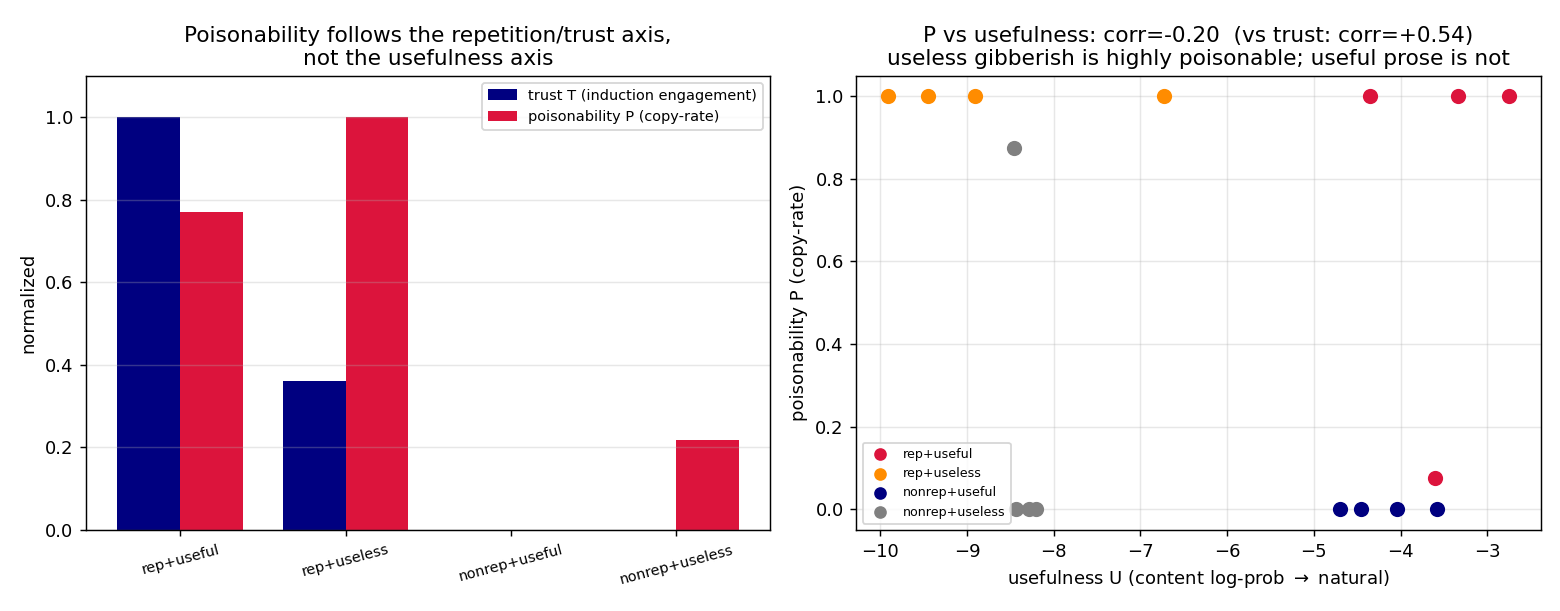
\includegraphics[width=\textwidth]{e4_trust.png}
\caption{E4-lite. \emph{Left:} per context type, trust $T$ and poisonability $P$ move together;
both ignore the usefulness columns. \emph{Right:} $P$ vs.\ usefulness---useless gibberish
($U\!\approx\!-9$) is fully poisonable while useful prose ($U\!\approx\!-4$) is not.
Reproduced by \texttt{experiments/e4\_trust.py}.}
\label{fig:e4}
\end{figure}

The dissociation is clean (Table~\ref{tab:e4}, Fig.~\ref{fig:e4}): \textbf{repetitive
gibberish---the \emph{least} useful content---is fully poisonable ($P{=}1.0$), while
non-repetitive real prose---useful---is not poisonable at all ($P{=}0.0$)}. This is the
real-transformer analogue of the toy's central finding and its defensive corollary: the
quantity to bound is \emph{trust on repeated/templated content}, independent of whether that
content is useful. (On a base model ``usefulness'' is a naturalness proxy, not a downstream
task; the instruction-tuned version is deferred to a larger machine.)

% ===========================================================================
\section{E5-lite: delivery from inside a document}\label{sec:e5}
% ===========================================================================
A scaled-down RAG attack (C5): a coherent prose document ($\sim$65 tokens) has an OOD payload
($p{=}3$) repeated $k$ times planted in it; we generate a continuation and measure
\emph{hijack} $=$ payload occupancy of the output. Two sweeps (Fig.~\ref{fig:e5}). \emph{Entry}
(placement, $k{=}8$): the payload hijacks \emph{only} when it sits at the very end
($\text{frac}{=}1.0\!\to\!0.52$); buried anywhere earlier it is $\approx 0$, even with just
$\sim$16 tokens of prose after it---sharper than E1.5's filler gap, because coherent prose
competes harder for the continuation. \emph{Lock-in} (repetitions, at the end): a clean knee
crossing $\tfrac12$ around $k\!\approx\!10$--$12$, \emph{higher} than the bare-context knee
($\sim$3): embedding in legitimate prose raises the poison cost.

\begin{figure}[t]
\centering
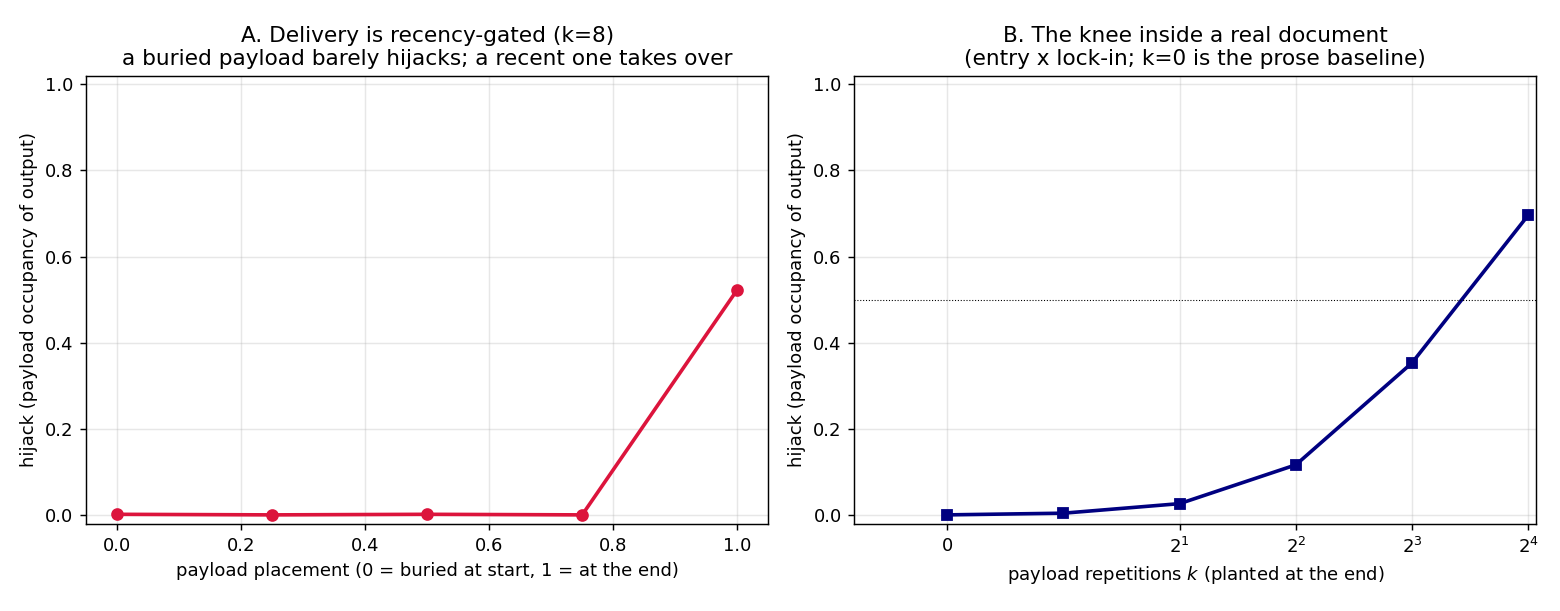
\includegraphics[width=\textwidth]{e5_hijack.png}
\caption{E5-lite. \emph{Left:} hijack vs.\ placement---delivery is recency-gated, only a payload
at the end takes over. \emph{Right:} hijack vs.\ repetitions at the end---the knee inside a real
document. Reproduced by \texttt{experiments/e5\_hijack.py}.}
\label{fig:e5}
\end{figure}

\textbf{C5 confirmed: hijack $=$ entry $\times$ lock-in.} Both must hold---the payload must be
recent \emph{and} repeated enough to overcome the legitimate content. The danger zone in a
long context is the span near where generation happens; burying a payload, or strong
surrounding context, suppresses the hijack.

% ===========================================================================
\section{E6: the context-window worm}\label{sec:e6}
% ===========================================================================
Transmission (C6): an infected host's output (containing the payload) becomes the next host's
context, passed as \emph{text} (decoded then re-tokenized, as agents and RAG pipelines pass
it); we count payload copies in each host's output across hops.

\begin{figure}[t]
\centering
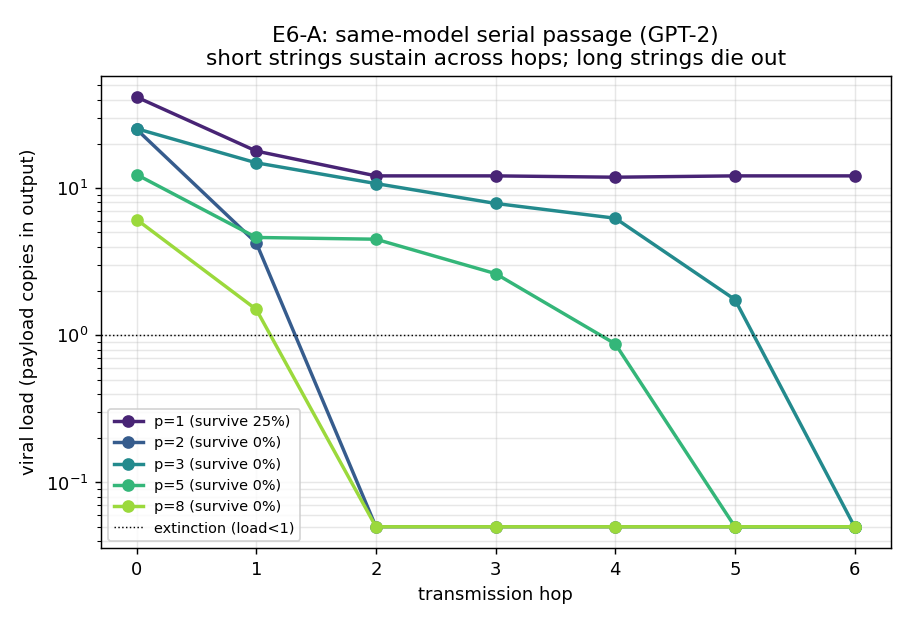
\includegraphics[width=0.49\textwidth]{e6_worm_serial.png}\hfill
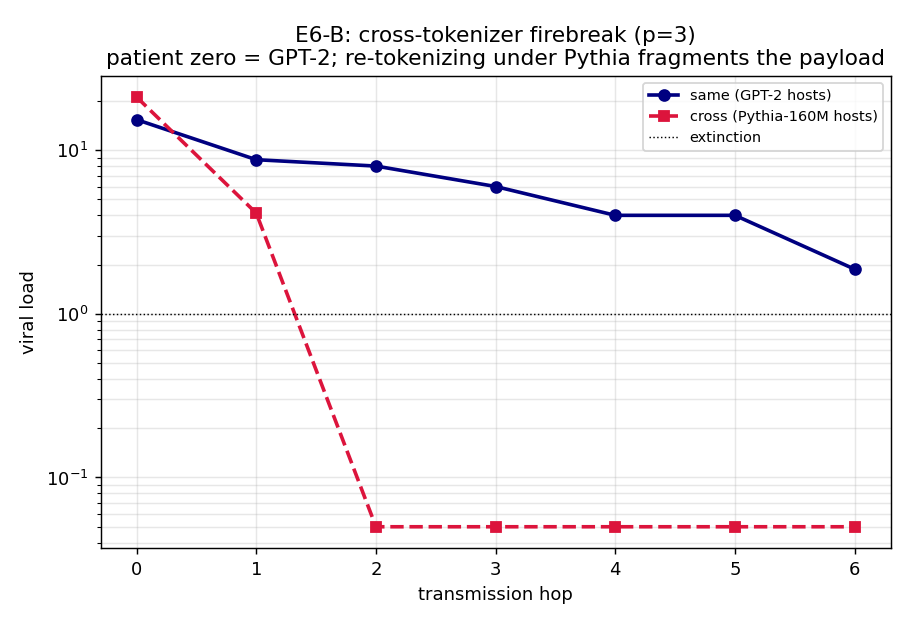
\includegraphics[width=0.49\textwidth]{e6_worm_crosstok.png}
\caption{E6. \emph{Left:} same-model serial passage---short strings ($p{=}1$) sustain at an
endemic load while longer strings die out, faster as $p$ grows (a critical length). \emph{Right:}
the cross-tokenizer firebreak---GPT-2$\to$GPT-2 transmission persists, GPT-2$\to$Pythia collapses
after one hop. Reproduced by \texttt{experiments/e6\_worm.py}.}
\label{fig:e6}
\end{figure}

\textbf{A real worm with a critical length.} In same-model serial passage (Fig.~\ref{fig:e6},
left), a length-1 string \emph{propagates indefinitely} at an endemic load ($\sim$12 copies/host)
while longer strings \emph{die out}, faster as $p$ grows (gone by hop 2 at $p{=}8$): the basic
reproduction number falls with string length and crosses $1$ around $p\!\approx\!1$--$2$,
exactly the toy's prediction (short $=$ epidemic, long $=$ one-shot). The epidemic is carried by
\emph{super-spreader} payloads that fully take over a host's output (occupancy $\to 1$, ending
mid-payload so the next host re-enters); most payloads reproduce weakly and die, tying the
critical length to the recency limit of E1.5. \textbf{Cross-tokenizer firebreak}
(Fig.~\ref{fig:e6}, right): same-tokenizer transmission survives to hop 6, but switching hosts
to Pythia-160M collapses it after one hop---re-tokenizing fragments the payload so induction
cannot copy it cleanly. A heterogeneous-model pipeline is naturally worm-resistant.

% ===========================================================================
\section{The paired detector}\label{sec:e7}
% ===========================================================================
The attacks of \S\ref{sec:e4}--\ref{sec:e6} all key on one quantity: the induction trust a
repeated span earns. The defense watches the same quantity. We score a context by its mean
\emph{induction engagement}---the attention the canonical induction heads (from E2) pay to
repeated-bigram continuations---which is high on a repeated/poisoned span and $\approx 0$ on
natural prose, regardless of whether the content is meaningful. As a binary detector (clean
prose documents vs.\ the same documents with an OOD payload repeated $k$ times), it separates
the two \emph{perfectly}: ROC-AUC $=1.0$ at every $k\in\{2,4,8,16\}$, with the score rising
monotonically in $k$ (Fig.~\ref{fig:e7}). It fires already at $k{=}2$, well below the
in-document hijack knee ($\sim$10--12, \S\ref{sec:e5}): it flags the poisonable configuration
\emph{before} it is dangerous, and on the trust signal independent of usefulness.

\begin{figure}[t]
\centering
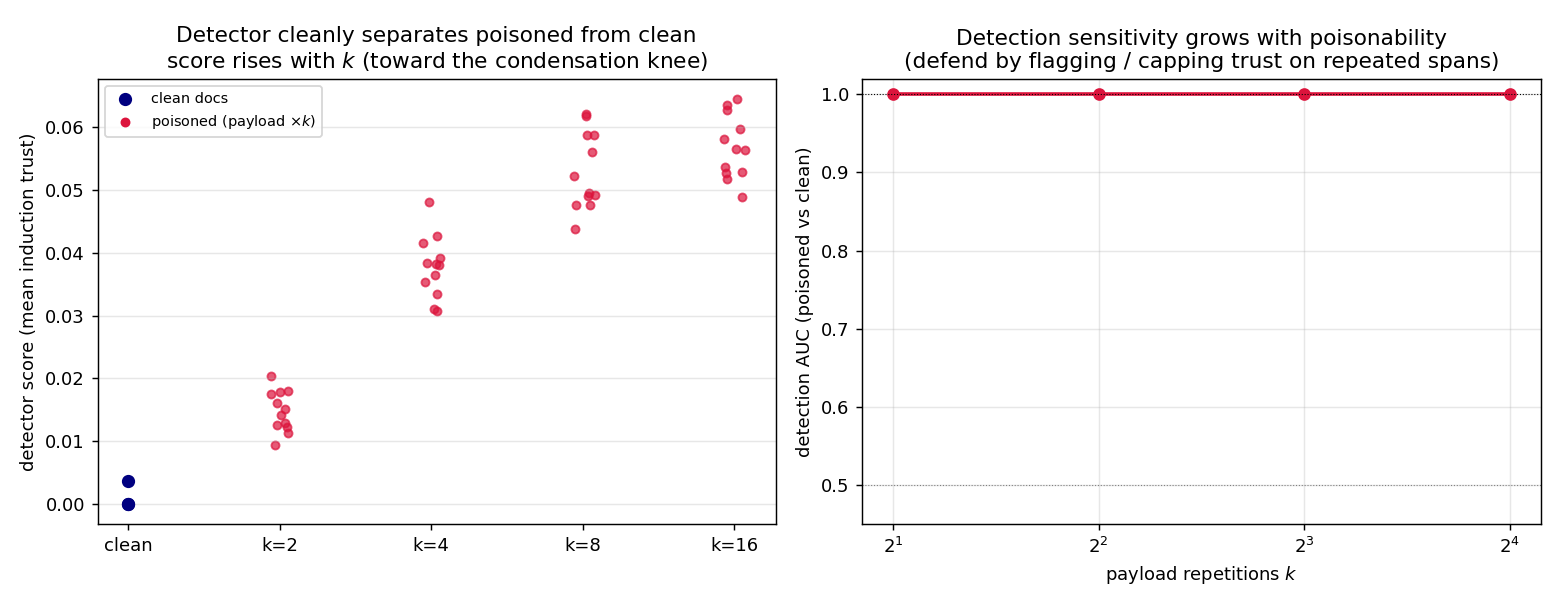
\includegraphics[width=\textwidth]{e7_detector.png}
\caption{The detector. \emph{Left:} score (mean induction trust) for clean docs vs.\ docs with
a payload repeated $k$ times---clean sits at $\approx 0$, poisoned rises with $k$. \emph{Right:}
detection AUC vs.\ $k$ ($=1.0$ throughout). Reproduced by \texttt{experiments/e7\_detector.py}.}
\label{fig:e7}
\end{figure}

Flagging---or capping the trust earned by---repeated spans that approach the condensation knee
is precisely what neutralizes the E5 hijack and the E6 worm; it is the transformer realization
of the toy's defensive corollary, \emph{bound trust, not usefulness}. \emph{Caveat:} the
detector flags \emph{any} induction-engaging repeated span, malicious or benign (boilerplate,
templates, repeated instructions). That is the correct behavior under the thesis---such spans
are genuinely poisonable (\S\ref{sec:e4})---but it identifies the poisonable \emph{configuration},
not malicious \emph{intent}, so a deployment needs a benign-repetition allowlist or a trust cap
rather than a hard block.

% ===========================================================================
\section{Threats to validity}\label{sec:threats}
% ===========================================================================
Beyond the small scale (one model, $R\!\sim\!4$--$6$ payloads, $\sim\!72$--$128$ samples per
cell, sampled $T{=}1.0$ only), the standing concerns are: \textbf{tokenization}---length is
in tokens and OOD spans tokenize unstably, addressed by a round-trip-stability filter;
\textbf{decoding}---the knee persists under \emph{greedy} decoding (with lower $N^*$, less
sampling noise to break reproduction), so it is a model property, not a sampling artifact; a
full temperature sweep is still future work; \textbf{instruction-tuned models} may comment or
refuse rather than copy, so
base models are used for the clean mechanism and chat models are a separate condition---now
run (E1.4, \S\ref{sec:scale}), where the knee persists with only a modest threshold rise;
\textbf{context-length vs.\ $N$}---addressed by E1.5 (\S\ref{sec:e15}): the knee
persists at fixed total length, so it is an $N$ effect, though reproduction is
distance-sensitive; and \textbf{scale}---the behavioral knee now extends cleanly to 7B across four families and is
flat with size (\S\ref{sec:scale}); what is still pending is the \emph{mechanistic}
attribution at scale (E2 on a $\ge$24\,GB GPU).

% ===========================================================================
\section{What is established, and what is not}\label{sec:honesty}
% ===========================================================================
On GPT-2-small, with controls and confidence intervals: a repeated out-of-distribution
string is regenerated past a sharp condensation knee (C1); the knee \emph{decreases} with
string length, the induction-like length-robustness predicted by the toy (C3); the knee is a
repetition effect (not context length) though distance-sensitive (E1.5); reproduction is a
cue-triggered copy rather than a frequency bias (C2, behaviorally); and---the new result---
ablating the canonical GPT-2 induction heads \emph{causally} collapses reproduction near the
knee, far beyond random-head damage, so \textbf{C2 is mechanistically established} on this
model (E2). The downstream claims also hold on GPT-2-small: poisonability is dissociated from
usefulness and aligned with induction trust (C4, \S\ref{sec:e4}); a planted span hijacks
generation as entry$\,\times\,$lock-in (C5, \S\ref{sec:e5}); and the worm has a critical string
length and a cross-tokenizer firebreak (C6, \S\ref{sec:e6}). The phenomena replicate in a second
model family (Pythia-160M). So all six conjectures C1--C6 have a qualitative real-transformer
result, and a paired detector (\S\ref{sec:e7}) realizes the toy's bound-trust defense (poisoned
vs.\ clean documents separate at AUC $1.0$ on the induction-trust signal). The keystone now also holds \emph{at scale}: the condensation knee is low and length-robust
from 355M to 7B across four model families and flat in parameter count (\S\ref{sec:scale}),
and it persists in instruction-tuned models---chat models copy rather than refuse, with only a
modest threshold rise (E1.4). What is \emph{not} yet established is the \textbf{mechanism at
scale}: whether induction-head ablation collapses reproduction on the larger models as it does
on GPT-2-small (E2 needs a $\ge$24\,GB GPU), together with the worm's critical length and
induction range at scale, the larger-context retrieval-grounded versions of C5 and C6, a
real-task (not naturalness-proxy) usefulness for C4, and the coherent self-extraction capstone
(E8). Those are the 24\,GB-GPU stage, now under way.

\begin{thebibliography}{9}
\bibitem{shumow2026trust} D.\ Shumow. \emph{Trust Is the Attack Surface: A Cryptanalytic
Reading of In-Context Memory Poisoning in a Markov Mixture Model.} Project
\texttt{trust-is-the-attack-surface}, 2026.

\bibitem{shumow2026contagion} D.\ Shumow. \emph{Contagious Context: Self-Reproducing and
Transmissible Token Strings in a Markov Cache.} Project
\texttt{trust-is-the-attack-surface}, 2026.

\bibitem{olsson2022} C.\ Olsson et al. \emph{In-context Learning and Induction Heads.}
Transformer Circuits, 2022.

\bibitem{bietti2023} A.\ Bietti, V.\ Cabannes, D.\ Bouchacourt, H.\ J\'egou, L.\ Bottou.
\emph{Birth of a Transformer: A Memory Viewpoint.} NeurIPS, 2023.

\bibitem{cohen2024} S.\ Cohen, R.\ Bitton, B.\ Nassi. \emph{Here Comes the AI Worm:
Unleashing Zero-click Worms that Target GenAI-Powered Applications.} 2024.

\bibitem{greshake2023} K.\ Greshake et al. \emph{Not What You've Signed Up For:
Compromising Real-World LLM-Integrated Applications with Indirect Prompt Injection.}
AISec, 2023.

\bibitem{radford2019} A.\ Radford, J.\ Wu, R.\ Child, D.\ Luan, D.\ Amodei, I.\ Sutskever.
\emph{Language Models are Unsupervised Multitask Learners.} OpenAI, 2019.
\end{thebibliography}

\end{document}
